
\documentclass[letterpaper,hide notes,xcolor={table,svgnames},pdftex]{beamer}
\def\showexamples{t}


%\usepackage[svgnames]{xcolor}

%% Demo talk
%\documentclass[letterpaper,notes=show]{beamer}

\usecolortheme{crane}%seahorse crane
\setbeamertemplate{navigation symbols}{}

\usetheme{MyPittsburgh}
%\usetheme{Frankfurt}

%\usepackage{tipa}

\usepackage{hyperref}
\usepackage{graphicx,xspace}
\usepackage[normalem]{ulem}

\newcommand\SF[1]{$\bigstar$\footnote{SF: #1}}

\usepackage{paratype}
\renewcommand*\familydefault{\sfdefault} %% Only if the base font of the document is to be sans serif
\usepackage[zerostyle=c]{newtxtt}
\usepackage[T1]{fontenc}

\newcounter{tmpnumSlide}
\newcounter{tmpnumNote}

\usepackage{xcolor}
\usepackage{tabu}
\definecolor{light-gray}{gray}{0.75}
\taburulecolor{light-gray}

% old question code
%\newcommand\question[1]{{$\bigstar$ \small \onlySlide{2}{#1}}}
% \newcommand\nquestion[1]{\ifdefined \presentationonly \textcircled{?} \fi \note{\par{\Large \textbf{?}} #1}}
% \newcommand\nanswer[1]{\note{\par{\Large \textbf{A}} #1}}


 \newcommand\mnote[1]{%
   \addtocounter{tmpnumSlide}{1}
   \ifdefined\showcues {~\tiny\fbox{\arabic{tmpnumSlide}}}\fi
   \note{\setlength{\parskip}{1ex}\addtocounter{tmpnumNote}{1}\textbf{\Large \arabic{tmpnumNote}:} {#1\par}}}

\newcommand\mmnote[1]{\note{\setlength{\parskip}{1ex}#1\par}}

%\newcommand\mnote[2][]{\ifdefined\handoutwithnotes {~\tiny\fbox{#1}}\fi
% \note{\setlength{\parskip}{1ex}\textbf{\Large #1:} #2\par}}

%\newcommand\mnote[2][]{{\tiny\fbox{#1}} \note{\setlength{\parskip}{1ex}\textbf{\Large #1:} #2\par}}

\newcommand\mquestion[2]{{~\color{red}\fbox{?}}\note{\setlength{\parskip}{1ex}\par{\Large \textbf{?}} #1} \note{\setlength{\parskip}{1ex}\par{\Large \textbf{A}} #2\par}\ifdefined \presentationonly \pause \fi}

\newcommand\blackboard[1]{%
\ifdefined   \showblackboard
  {#1}
  \else {\begin{center} \fbox{\colorbox{blue!30}{%
         \begin{minipage}{.95\linewidth}%
           \hspace{\stretch{1}} Some space intentionally left blank; done at the blackboard.%
         \end{minipage}}}\end{center}}%
         \fi%
}



%\newcommand\q{\tikz \node[thick,color=black,shape=circle]{?};}
%\newcommand\q{\ifdefined \presentationonly \textcircled{?} \fi}

\usepackage{listings}
\lstset{%
  keywordstyle=\bfseries,
  aboveskip=15pt,
  belowskip=15pt,
  captionpos=b,
  identifierstyle=\ttfamily,
  escapeinside={(*@}{@*)},
  stringstyle=\ttfamiliy,
  frame=lines,
  numbers=left, basicstyle=\scriptsize, numberstyle=\tiny, stepnumber=0, numbersep=2pt}

\usepackage{siunitx}
\newcommand\sius[1]{\num[group-separator = {,}]{#1}\si{\micro\second}}
\newcommand\sims[1]{\num[group-separator = {,}]{#1}\si{\milli\second}}
\newcommand\sins[1]{\num[group-separator = {,}]{#1}\si{\nano\second}}
\sisetup{group-separator = {,}, group-digits = true}

%% -------------------- tikz --------------------
\usepackage{tikz}
\usetikzlibrary{positioning}
\usetikzlibrary{arrows,backgrounds,automata,decorations.shapes,decorations.pathmorphing,decorations.markings,decorations.text}

\tikzstyle{place}=[circle,draw=blue!50,fill=blue!20,thick, inner sep=0pt,minimum size=6mm]
\tikzstyle{transition}=[rectangle,draw=black!50,fill=black!20,thick, inner sep=0pt,minimum size=4mm]

\tikzstyle{block}=[rectangle,draw=black, thick, inner sep=5pt]
\tikzstyle{bullet}=[circle,draw=black, fill=black, thin, inner sep=2pt]

\tikzstyle{pre}=[<-,shorten <=1pt,>=stealth',semithick]
\tikzstyle{post}=[->,shorten >=1pt,>=stealth',semithick]
\tikzstyle{bi}=[<->,shorten >=1pt,shorten <=1pt, >=stealth',semithick]

\tikzstyle{mut}=[-,>=stealth',semithick]

\tikzstyle{treereset}=[dashed,->, shorten >=1pt,>=stealth',thin]

\usepackage{ifmtarg}
\usepackage{xifthen}
\makeatletter
% new counter to now which frame it is within the sequence
\newcounter{multiframecounter}
% initialize buffer for previously used frame title
\gdef\lastframetitle{\textit{undefined}}
% new environment for a multi-frame
\newenvironment{multiframe}[1][]{%
\ifthenelse{\isempty{#1}}{%
% if no frame title was set via optional parameter,
% only increase sequence counter by 1
\addtocounter{multiframecounter}{1}%
}{%
% new frame title has been provided, thus
% reset sequence counter to 1 and buffer frame title for later use
\setcounter{multiframecounter}{1}%
\gdef\lastframetitle{#1}%
}%
% start conventional frame environment and
% automatically set frame title followed by sequence counter
\begin{frame}%
\frametitle{\lastframetitle~{\normalfont(\arabic{multiframecounter})}}%
}{%
\end{frame}%
}
\makeatother

\makeatletter
\newdimen\tu@tmpa%
\newdimen\ydiffl%
\newdimen\xdiffl%
\newcommand\ydiff[2]{%
    \coordinate (tmpnamea) at (#1);%
    \coordinate (tmpnameb) at (#2);%
    \pgfextracty{\tu@tmpa}{\pgfpointanchor{tmpnamea}{center}}%
    \pgfextracty{\ydiffl}{\pgfpointanchor{tmpnameb}{center}}%
    \advance\ydiffl by -\tu@tmpa%
}
\newcommand\xdiff[2]{%
    \coordinate (tmpnamea) at (#1);%
    \coordinate (tmpnameb) at (#2);%
    \pgfextractx{\tu@tmpa}{\pgfpointanchor{tmpnamea}{center}}%
    \pgfextractx{\xdiffl}{\pgfpointanchor{tmpnameb}{center}}%
    \advance\xdiffl by -\tu@tmpa%
}
\makeatother
\newcommand{\copyrightbox}[3][r]{%
\begin{tikzpicture}%
\node[inner sep=0pt,minimum size=2em](ciimage){#2};
\usefont{OT1}{phv}{n}{n}\fontsize{4}{4}\selectfont
\ydiff{ciimage.south}{ciimage.north}
\xdiff{ciimage.west}{ciimage.east}
\ifthenelse{\equal{#1}{r}}{%
\node[inner sep=0pt,right=1ex of ciimage.south east,anchor=north west,rotate=90]%
{\raggedleft\color{black!50}\parbox{\the\ydiffl}{\raggedright{}#3}};%
}{%
\ifthenelse{\equal{#1}{l}}{%
\node[inner sep=0pt,right=1ex of ciimage.south west,anchor=south west,rotate=90]%
{\raggedleft\color{black!50}\parbox{\the\ydiffl}{\raggedright{}#3}};%
}{%
\node[inner sep=0pt,below=1ex of ciimage.south west,anchor=north west]%
{\raggedleft\color{black!50}\parbox{\the\xdiffl}{\raggedright{}#3}};%
}
}
\end{tikzpicture}
}


%% --------------------

%\usepackage[excludeor]{everyhook}
%\PushPreHook{par}{\setbox0=\lastbox\llap{MUH}}\box0}

%\vspace*{\stretch{1}

%\setbox0=\lastbox \llap{\textbullet\enskip}\box0}

\setlength{\parskip}{\fill}

\newcommand\noskips{\setlength{\parskip}{1ex}}
\newcommand\doskips{\setlength{\parskip}{\fill}}

\newcommand\xx{\par\vspace*{\stretch{1}}\par}
\newcommand\xxs{\par\vspace*{2ex}\par}
\newcommand\tuple[1]{\langle #1 \rangle}
\newcommand\code[1]{{\sf \footnotesize #1}}
\newcommand\ex[1]{\uline{Example:} \ifdefined \presentationonly \pause \fi
  \ifdefined\showexamples#1\xspace\else{\uline{\hspace*{2cm}}}\fi}

\newcommand\ceil[1]{\lceil #1 \rceil}


\AtBeginSection[]
{
   \begin{frame}
       \frametitle{Outline}
       \tableofcontents[currentsection]
   \end{frame}
}



\pgfdeclarelayer{edgelayer}
\pgfdeclarelayer{nodelayer}
\pgfsetlayers{edgelayer,nodelayer,main}

\tikzstyle{none}=[inner sep=0pt]
\tikzstyle{rn}=[circle,fill=Red,draw=Black,line width=0.8 pt]
\tikzstyle{gn}=[circle,fill=Lime,draw=Black,line width=0.8 pt]
\tikzstyle{yn}=[circle,fill=Yellow,draw=Black,line width=0.8 pt]
\tikzstyle{empty}=[circle,fill=White,draw=Black]
\tikzstyle{bw} = [rectangle, draw, fill=blue!20, 
    text width=4em, text centered, rounded corners, minimum height=2em]
    
    \newcommand{\CcNote}[1]{% longname
	This work is licensed under the \textit{Creative Commons #1 3.0 License}.%
}
\newcommand{\CcImageBy}[1]{%
	\includegraphics[scale=#1]{creative_commons/cc_by_30.pdf}%
}
\newcommand{\CcImageSa}[1]{%
	\includegraphics[scale=#1]{creative_commons/cc_sa_30.pdf}%
}
\newcommand{\CcImageNc}[1]{%
	\includegraphics[scale=#1]{creative_commons/cc_nc_30.pdf}%
}
\newcommand{\CcGroupBySa}[2]{% zoom, gap
	\CcImageBy{#1}\hspace*{#2}\CcImageNc{#1}\hspace*{#2}\CcImageSa{#1}%
}
\newcommand{\CcLongnameByNcSa}{Attribution-NonCommercial-ShareAlike}


\newenvironment{changemargin}[1]{% 
  \begin{list}{}{% 
    \setlength{\topsep}{0pt}% 
    \setlength{\leftmargin}{#1}% 
    \setlength{\rightmargin}{1em}
    \setlength{\listparindent}{\parindent}% 
    \setlength{\itemindent}{\parindent}% 
    \setlength{\parsep}{\parskip}% 
  }% 
  \item[]}{\end{list}} 




\title{Lecture 25 --- The Linked List}

\author{J. Zarnett\\
\texttt{jzarnett@uwaterloo.ca}}
\institute{Department of Electrical and Computer Engineering \\
  University of Waterloo}
\date{\today}

\begin{document}

\begin{frame}
  \titlepage
  
  \begin{center}
  \small{Acknowledgments: W.D. Bishop}
  \end{center}
\end{frame}

\begin{frame}
\frametitle{Arrays and Collections}
We've established that we would like to have a dynamic collection that does not rely on an array.

When using an array, we have a reference to the array.\\
\quad The reference tells us where the start of the array is in memory.\\
\quad The index tells us which entry of the array to access.

In a collection, the array serves the purpose of keeping the elements next to one another so that we can move from one to the next.\\
\quad To find the next object in an array, we increment the index by 1.

\end{frame}

\begin{frame}
\frametitle{Linking Collection Elements}
If the elements are not stored in an array, given that we know where the first object is, how might we get to the next object?

Idea: use a reference to link the objects together.

In the simplest case, each object has a reference to the next object.\\
\quad A null reference indicates there is no next object.

Analogy: pirate treasure map.\\
\quad Follow the map's directions; it leads to treasure and another map.\\
\quad The 2$^{nd}$ map says how to find another treasure and a third map.\\
\quad ... and repeat until we get to the final treasure (that has no map).

\end{frame}

\begin{frame}
\frametitle{The Linked List}

Linked lists are similar in function to arrays but are more flexible:
\begin{itemize}
    \item The size of a linked list is not fixed
    \item Objects may be easily inserted or deleted from a linked list
    \item Objects may be sorted (if desired)
\end{itemize}

Linked lists are formed using self-referential structs (or later, classes):\\
\quad A data type that has a pointer to another item of the same type.

For example, a class \texttt{ListEntry} can contain one or more data fields as well as a reference to another object of type \texttt{ListEntry}.

\end{frame}


\begin{frame}[fragile]
\frametitle{Linking Objects}

Let's write a very simple \texttt{list\_entry} struct.

\begin{verbatim}
struct list_entry
{
    int data;
    list_entry* next;
}
\end{verbatim}

This works because \texttt{next} is a pointer.

The compiler can figure out how much memory \texttt{list\_entry} needs because it knows the size of an \texttt{int} and the size of a pointer (\texttt{next}).

\end{frame}

\begin{frame}
\frametitle{Creating a List of Integers}

Using the struct previously defined, it is possible to create a collection of records known as a singly linked list.

For example, it is possible to define a list containing a set of integers \{3,1,6\} as follows:

\begin{center}
    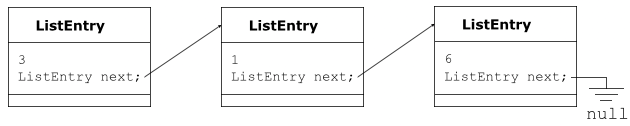
\includegraphics[width=\textwidth]{images/list316.png}
\end{center}

When a pointer is null, it is sometimes drawn as if it's an electrical connection to ground.

\end{frame}

\begin{frame}
\frametitle{Accessing the Linked List}
The linked list on the previous slide has no references pointing to it...

Developers often keep a pointer to the head and the tail of the list:

\begin{center}
    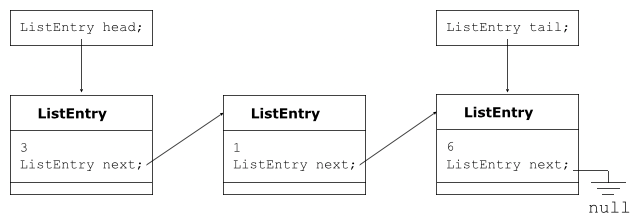
\includegraphics[width=\textwidth]{images/listheadtail.png}
\end{center}

A tail pointer is not strictly needed; it's a perfectly functional linked list with only a head reference. A tail poster can be convenient.

\end{frame}


\begin{frame}[fragile]
\frametitle{The \texttt{linked\_list}}

\begin{verbatim}
struct linked_list {
    list_entry* head;
    list_entry* tail;
}
\end{verbatim}

This is certainly a simple definition...

Now, how about some functions to manipulate it:
\texttt{
\begin{itemize}
	\item initialize
	\item append
	\item prepend
	\item remove\_first
	\item clear
\end{itemize}
}

\end{frame}

\begin{frame}[fragile]
\frametitle{Initialize}

\begin{verbatim}
void initialize( linked_list* list ) {
    list->head = 0;
    list->tail = 0;
}
\end{verbatim}

\end{frame}

\begin{frame}[fragile]
\frametitle{Append}

\begin{verbatim}
void append( linked_list* list, int data ) {
    if (tail == 0) {
        list->head = new list_entry;
        list->tail = head;
        list->tail->data = data;
        list->tail->next = 0;
    } else { 
        list_entry* entry = new list_entry;
        entry->data = data;
        entry->next = 0;
        list->tail.next = entry;
        list->tail = tail->next;
    }
}
\end{verbatim}

\end{frame}

\begin{frame}[fragile]
\frametitle{Prepend}

\begin{verbatim}
void prepend( linked_list* list, int data ) {
   list_entry* tmp = new list_entry;
   tmp->data = data;
   tmp->next = list->head;
   
   list->head = tmp;
   if (list->tail == 0) {
       list->tail = list->head;
   }
}
\end{verbatim}

\end{frame}

\begin{frame}[fragile]
\frametitle{Remove First}

\begin{verbatim}
list_entry* remove_first( linked_list* list ) {
    list_entry* result = list->head;
    if (list->head != 0) {
        list->head = list->head->next;
    }
    if (list->head == 0) {
        list->tail = 0;
    }
    return result;
}
\end{verbatim}

\end{frame}


\begin{frame}[fragile]
\frametitle{Clear}

\begin{verbatim}
void clear( linked_list* list ) {
   while( list-> head != 0 ) {
       list_entry* current = list->head;
       list->head = list->head->next;
       delete current;	
   }
   list->tail = 0;
}
\end{verbatim}

\end{frame}


\begin{frame}
\frametitle{List Creation Demonstration}

Let's work with this code and represent visually what the following series of statements would look like when executed.

\texttt{
\begin{enumerate}
	\item initialize( list );
	\item append( list,  3 );
	\item append( list,  1 );
	\item append( list,  6 );
	\item prepend( list,  4 );
	\item prepend( list,  5 );
	\item remove\_first( list );
	\item prepend( list,  2 );
	\item clear( list );
\end{enumerate}
}

[Demo done on the board to facilitate understanding.]

\end{frame}


\begin{frame}
\frametitle{Expanding on the Simple Linked List}

A second reference in each \texttt{list\_entry} that refers to the previous element can simplify deletion and other complex operations.\\
\quad This is known as a doubly-linked list.

The use of dummy items (i.e., dummy head or dummy tail) can simplify some the termination conditions for some loops.

A dummy item is a \texttt{list\_entry} that has a valid reference but never any valid data. It is constructed when the list is constructed.

A length member field can be added to keep track of the length of the list as items are added and removed.

\end{frame}

\end{document}

